\documentclass[xcolor=svgnames,17pt]{beamer}

\usepackage[export]{adjustbox}
\usepackage{bashful}
\usepackage{bookmark}
\usepackage{colortbl} \arrayrulecolor[gray]{0.7}
\usepackage{microtype}
\usepackage{pgfpages}
\usepackage{rotating}
\usepackage{textcomp}
\usepackage{tabularx}
\usepackage{xspace}
\usepackage{verbatim}

\usepackage{fontspec}

\hypersetup{pdfpagemode=,colorlinks=true,urlcolor=blue}

%\urlstyle{same}

\newcommand*{\sizefont}[1]{%
    \ifcase#1\relax
    \or \tiny
    \or \scriptsize
    \or \footnotesize
    \or \small
    \or \normalsize
    \or \large
    \or \Large
    \or \LARGE
    \or \huge
    \or \Huge
    \fi}

%%

\newcommand*{\mybullet}{\tikz[baseline=-.6ex]\node[%
    draw,circle,inner sep = -0.15ex,fill]{.};\xspace}

%\setbeamertemplate{footline}{
%    \usebeamercolor[fg]{page number in head/foot}%
%    \usebeamerfont{page number in head/foot}%
%    \hspace*{1ex}\insertframenumber\,/\,\inserttotalframenumber\hfill
%    github.com/andrewdotn/...\ }

\newcommand*{\plainfooter}{%
    \setbeamertemplate{footline}{
        \usebeamercolor[fg]{page number in head/foot}%
        \usebeamerfont{page number in head/foot}%
        \hspace*{1ex}\insertframenumber\,/\,\inserttotalframenumber\vskip2pt}}

\makeatletter
\def\alphslide{\@alph{\intcalcAdd{1}{\intcalcSub{\thepage}{\beamer@framestartpage}}}}
\newcommand*{\plainstepfooter}{
    \setbeamertemplate{footline}{
        \usebeamercolor[fg]{page number in head/foot}%
        \usebeamerfont{page number in head/foot}%
        \hspace*{1ex}\insertframenumber\alphslide\,/\,\inserttotalframenumber\vskip2pt}}
\makeatother

\setbeamertemplate{note page}{
    \sizefont{3}
    \setlength{\parskip}{10pt}
    \insertnote
    \par}

\setbeamertemplate{navigation symbols}{}
\setbeamerfont{title}{size=\LARGE}
\setbeamerfont{frametitle}{size=\LARGE}
\setbeamerfont{framesubtitle}{size=\normalsize}

\newcommand*{\tocsection}[1]{\pdfbookmark[2]{#1}{#1}}

\lstdefinestyle{bashfulStdout}{
    basicstyle=\ttfamily,
    keywords={},
    showstringspaces=false
}%

%%

\title{git init}

\author{\texorpdfstring{%
    Andrew Neitsch}{Andrew Neitsch}}

\date{\small 2018-01-24}

\begin{document}

\tocsection{Title page}

\sizefont{4}

\begin{frame}[plain]
\titlepage
\end{frame}

\begin{frame}{Outline}
\tableofcontents
\end{frame}

\section{Version control}

\def\fillinblank{\_\_\_\_}

\begin{frame}{What is version control?}
a system for storing source code
\\[\baselineskip] \pause

where every code change is a distinct entity called a \textit{commit}
\\[\baselineskip] \pause

where every commit has an attached record of who made the change, when they
made it, and why they said they made the change
\end{frame}

\begin{frame}[fragile]{Example}
\href{https://github.com/python/cpython/commit/5382c05021026fe623def829d121f5f6af4909fb}{github.com/python/cpython/5382c05}

\sizefont{1}
\begin{verbatim}
Author: Andrew Svetlov <andrew.svetlov@gmail.com>
Date:   Sun Dec 17 16:41:30 2017 +0200

    bpo-32351: Use fastpath in asyncio.sleep if delay<0 (#4908)
    
    * Use fastpath in asyncio.sleep if delay<0
    
    * Add NEWS entry

diff Lib/asyncio/tasks.py
@@ -503,7 +503,7 @@ def __sleep0():
 
 async def sleep(delay, result=None, *, loop=None):
     """Coroutine that completes after a given time (in seconds)."""
-    if delay == 0:
+    if delay <= 0:
         await __sleep0()
         return result
 
new file Misc/NEWS.d/next/Library/2017-12-17-14-23-23.bpo-32351.95fh2K.rst
@@ -0,0 +1 @@
+Use fastpath in asyncio.sleep if delay<0 (2x boost)

\end{verbatim}
\end{frame}

\begin{frame}{Benefits of version control}
\begin{itemize}
\only<1->{\item \textbf{diff}} \only<1>{show you what you’ve change so you
can review it}
\only<2->{\item \textbf{backups and undo}} \only<2>{you can go back to a
known good state, or selectively revert a specific change, if things start
crashing, or an idea turns out not to work}
\only<3->{\item \textbf{history}} \only<3>{you can safely delete code you
don’t need right now to keep things clean, knowing you can get it back any
time}
\only<4->{\item \textbf{context}} \only<4>{commit messages can explain
design decisions, link to bug reports, or, even if blank, tell you who to
ask for help}
\only<5->{\item \textbf{merges}} \only<5>{if you make unrelated changes to
different files, the version control system will merge them instead of
overwriting}
\only<6->{\item \textbf{synchronization}} \only<6>{synchronizing your
version of the code with someone else only requires sending recent changes,
not the complete source code}
\only<7->{\item \textbf{bisect}} \only<7>{find sources of bugs by checking
different versions to see when the bug first shows up}
% https://bugs.kde.org/show_bug.cgi?id=161174
\end{itemize}
\only<8>{In short, there are tons of benefits}
\end{frame}

\begin{frame}{Is it worth the effort?}
\pause
\begin{itemize}
\item Indispensable when working with others, for automatic merges alone.
The alternative is complete chaos.
\pause
\item Useful even if the only other people working on the project are past you
  and future you\pause\\
  “This was working 10 minutes ago. What did I just change?”
\end{itemize}
\end{frame}

\section{Version control with git}

\begin{frame}
\tableofcontents[currentsection]
\end{frame}

\begin{frame}{GitHub does all of that with a nice web UI}
\only<1>{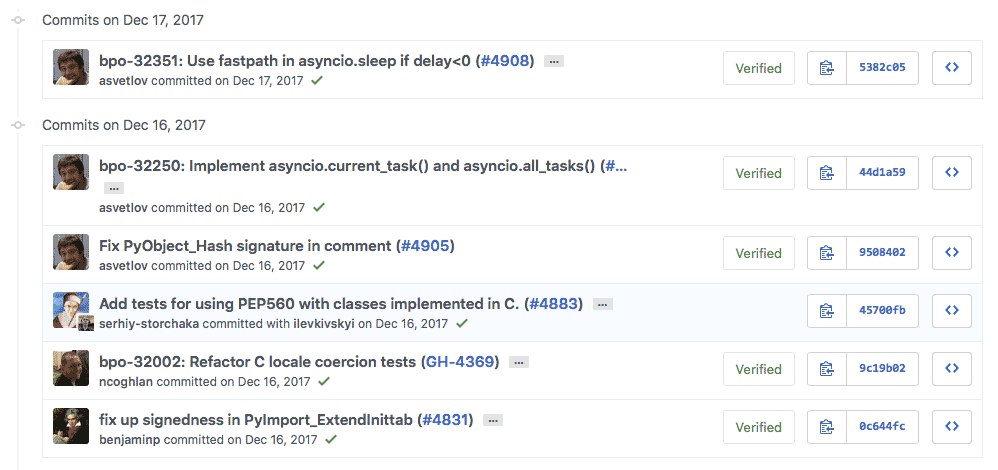
\includegraphics[width=\paperwidth,center]{github-commitlog.png}}
\only<2>{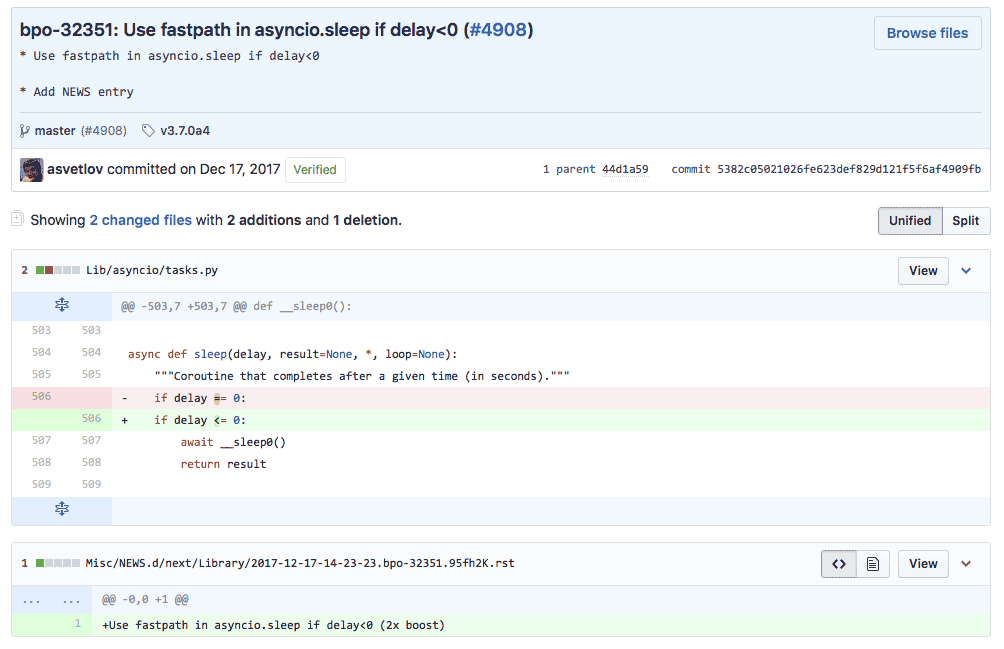
\includegraphics[width=\paperwidth,center]{github-commitdetails.png}}
\only<3>{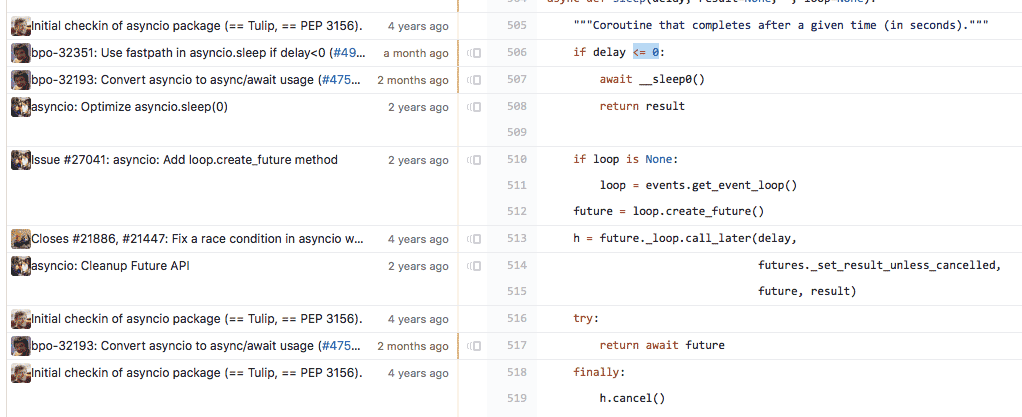
\includegraphics[width=\paperwidth,center]{github-annotate.png}}
\end{frame}

\begin{frame}[fragile]{But to use GitHub \\ you have to use git}
\texttt{
\$ git help \\
usage: git [--version] [--help] [-C <path>] [-c name=value]
           [--exec-path[=<path>]] [--html-path] [--man-path] [--info-path]
           [-p | --paginate | --no-pager] [--no-replace-objects] [--bare]
           [--git-dir=<path>] [--work-tree=<path>] [--namespace=<name>]
           <command> [<args>]
}
\end{frame}

\begin{frame}{What is git?}
\begin{itemize}
\only<1-5>{\item Open-source version control system}
\only<2-3>{\item Originally written in 2005 by Linus Torvalds, creator of
Linux, to store Linux source code}
\only<3>{\item Target audience is C programmers who work on the linux kernel}
\only<4->{\item git can get very complicated, very quickly}
\only<5-6>{\item I used to use Mercurial, which is written in Python, and is
a lot friendlier} \only<6>{and less popular}
\end{itemize}
\only<7>{
\begin{columns}
\column{.4\textwidth}
\fbox{%
    
\includegraphics[width=\textwidth]{version-control-with-git.jpg}}
\column{.6\textwidth}
There is an O’Reilly book:
\href{https://www.safaribooksonline.com/library/view/version-control-with/9781449345037/}{Version Control with Git}
\end{columns}
}
\only<6>{
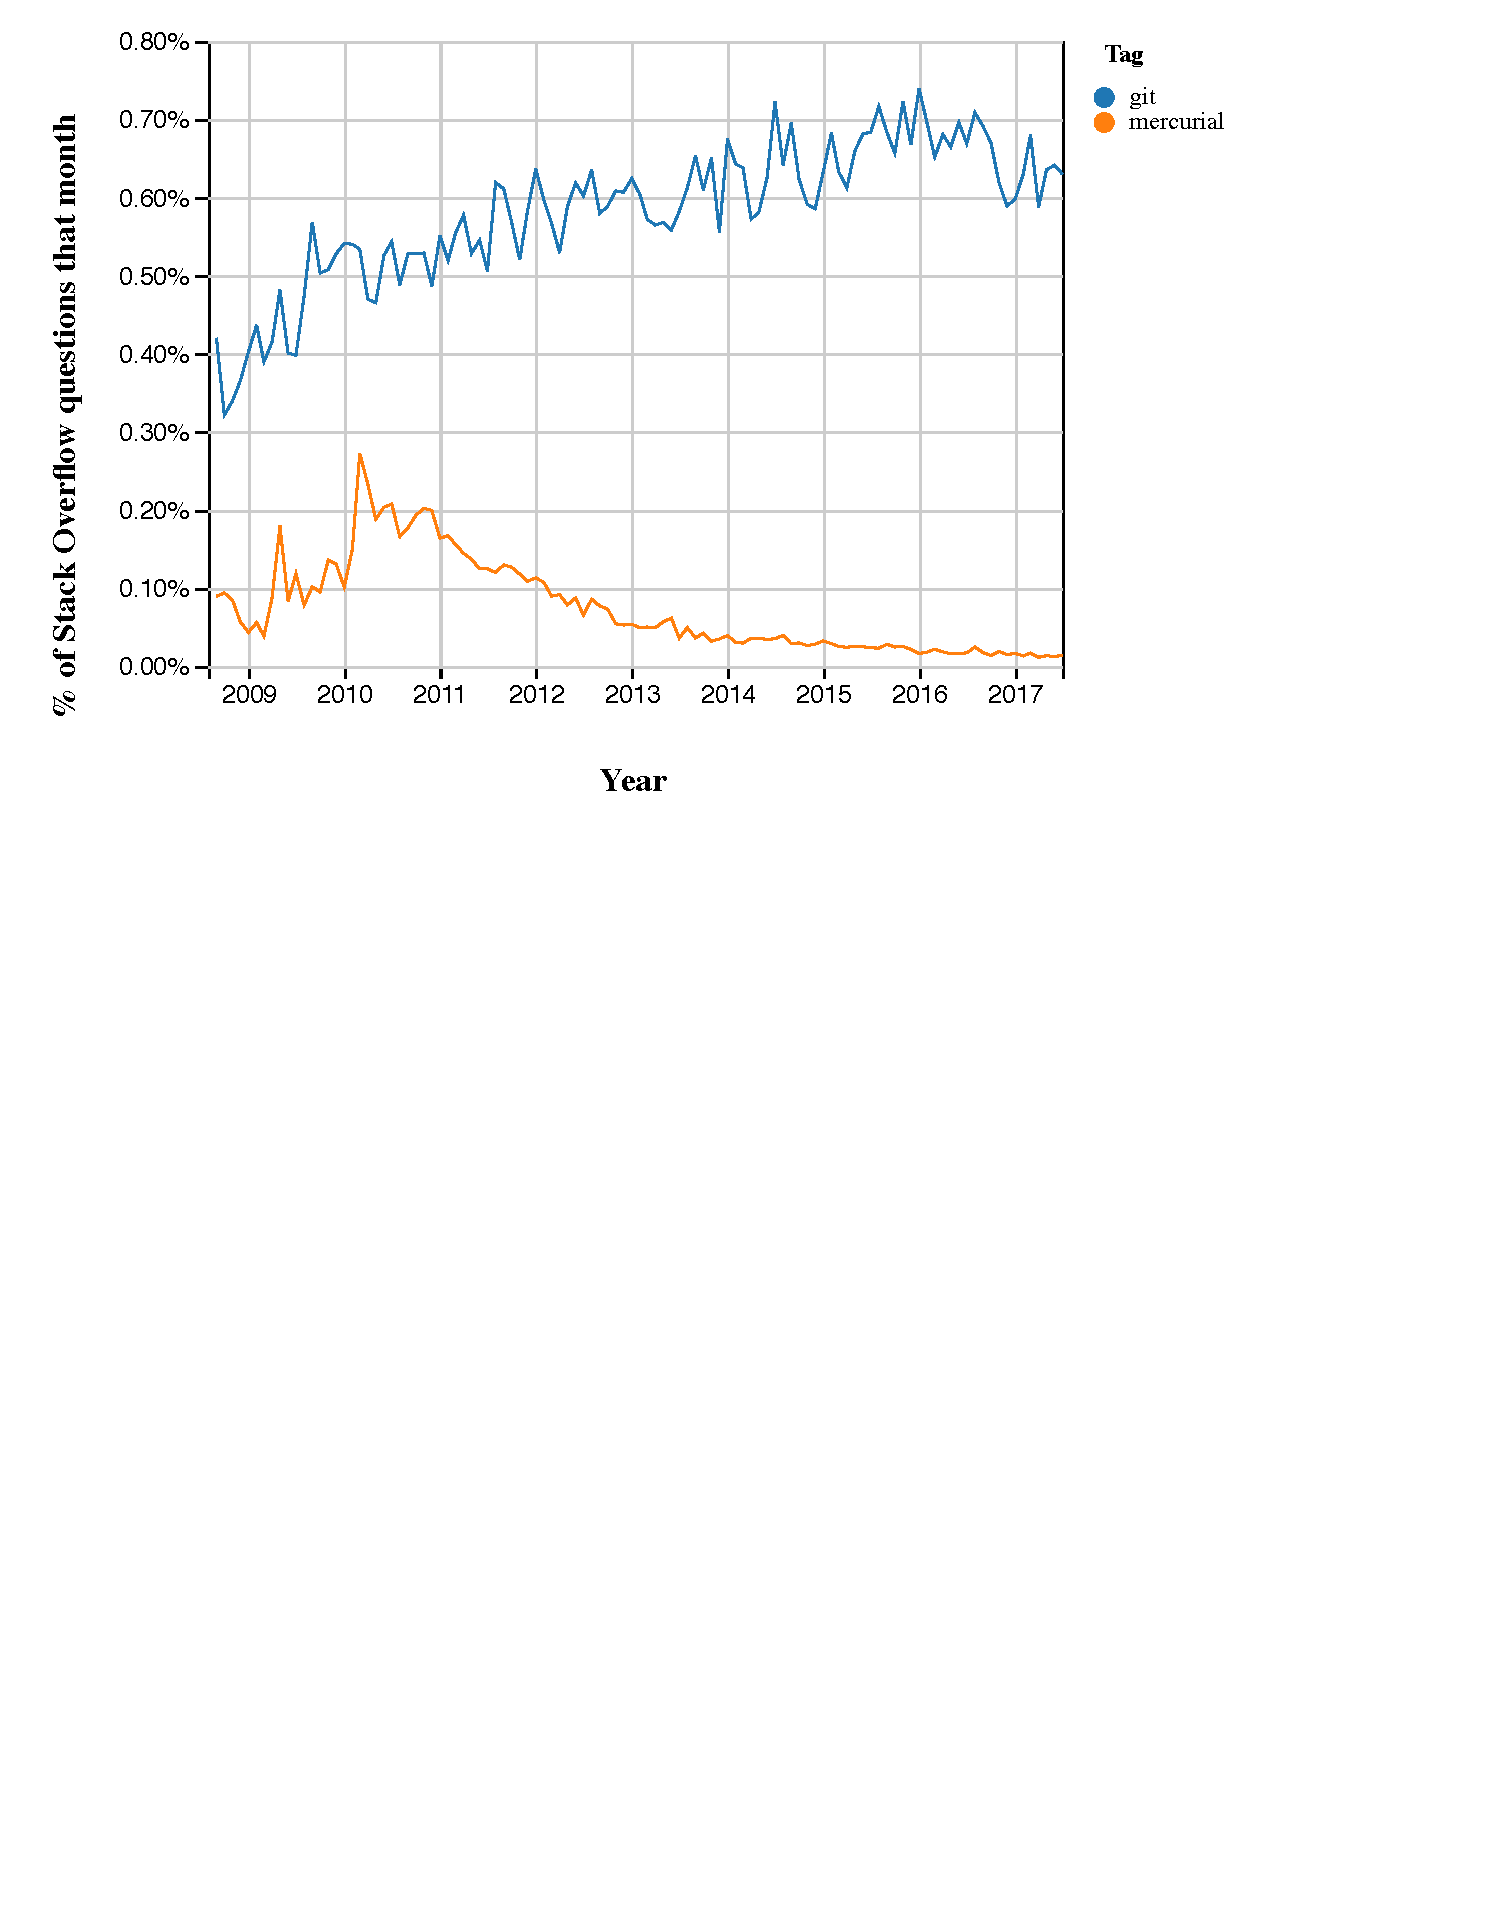
\includegraphics[width=0.5\paperwidth,center]{git-vs-hg.pdf}\\
\href{https://insights.stackoverflow.com/trends?tags=git,mercurial}{
insights.stackoverflow.com/trends?tags=git,mercurial}}
\end{frame}

\begin{frame}[fragile]{Basic config}
\begin{verbatim}
$ cat ~/.gitconfig

[user]
  name = First Last
  email = first@last.ca

[commit]
  # Show diff preview in commit message editor
  verbose = true

[merge]
  # Include common ancestor in merge conflicts
  conflictstyle = diff3

\end{verbatim}
\end{frame}

\begin{frame}[fragile]{Walk through: init and status}
\sizefont{2}
\begin{verbatim}
$ git init
Initialized empty Git repository in /path/to/whatever/.git
\end{verbatim}
\pause
\begin{verbatim}
$ echo hi > foo
$ git status
On branch master

Initial commit

Untracked files:
  (use "git add <file>..." to include in what will be committed)

	foo

nothing added to commit but untracked files present
(use "git add" to track)
\end{verbatim}
\end{frame}

\begin{frame}[fragile]{Walk through: add}
\sizefont{2}
\begin{verbatim}
$ git init
Initialized empty Git repository in /path/to/whatever/.git
$ echo hi > foo
\end{verbatim}
\begin{verbatim}
$ git add foo
$ git status
On branch master

Initial commit

Changes to be committed:
  (use "git rm --cached <file>..." to unstage)

	new file:   foo

\end{verbatim}
\end{frame}

\begin{frame}[fragile]{Walk through: commit}
\sizefont{1}
\begin{verbatim}
$ git commit
\end{verbatim}
\pause
\begin{verbatim}
Add foo
# Please enter the commit message for your changes. Lines starting
# with '#' will be ignored, and an empty message aborts the commit.
# Explicit paths specified without -i or -o; assuming --only paths...
# On branch master
#
# Initial commit
#
# Changes to be committed:
#	new file:   foo
#
# ------------------------ >8 ------------------------
# Do not touch the line above.
# Everything below will be removed.
diff --git a/foo b/foo
new file mode 100644
index 0000000..ce01362
--- /dev/null
+++ b/foo
@@ -0,0 +1 @@
+hello
~
~
\end{verbatim}
\end{frame}

\begin{frame}[fragile]{Walk through: log}
\sizefont{2}
\begin{verbatim}
$ git init
$ echo hello > foo
$ git add foo
$ git commit
\end{verbatim}
\pause
\begin{verbatim}
$ git log -p

commit 61c1f88999741f5feae711911b74ee6b21e954cd (HEAD -> master)
Author: Andrew <andrew@example.org>
Date:   Fri Jan 5 04:25:15 2018 -0700

    Add foo

diff --git a/foo b/foo
new file mode 100644
index 0000000..45b983b
--- /dev/null
+++ b/foo
@@ -0,0 +1 @@
+hi
\end{verbatim}
\end{frame}

\begin{frame}{Connecting to GitHub}
\begin{itemize}
\item \href{https://github.com/new}{https://github.com/new}
\pause
\item \texttt{git remote add github.com/\$you/\$repo
https://github.com/\$you/\$repo.git}
\pause
\item \texttt{git push github.com/\$you/\$repo}
\pause
\item \sizefont{2} you can use SSH too, but that’s another talk
\end{itemize}
\end{frame}

\begin{frame}{Working with friends}
\begin{itemize}
\item You can give others write access to your repositories \\
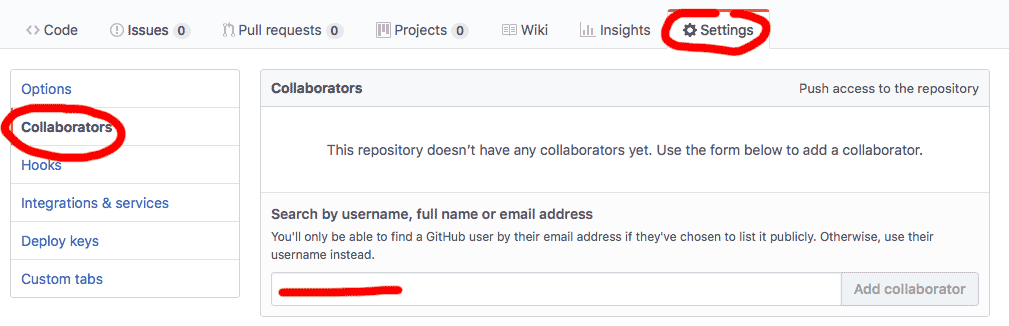
\includegraphics[width=\paperwidth,center]{github-add-collaborator.png}
\item Then \texttt{git push} and \texttt{git pull}
\end{itemize}
\end{frame}

\begin{frame}[fragile]{Merge conflicts}
\sizefont{2}
\begin{verbatim}
$ git pull
Auto-merging foo
\end{verbatim}
\pause
\begin{verbatim}
CONFLICT (content): Merge conflict in foo
Automatic merge failed; fix conflicts and then commit the result.
$ cat foo
<<<<<<< HEAD
hello there
||||||| merged common ancestors
hello
=======
goodbye
>>>>>>> 99f9df7
\end{verbatim}
\pause
\begin{verbatim}
$ echo goodbye there > foo
$ git add foo
$ git commit -m 'Fix merge conflict'
\end{verbatim}
\end{frame}

\begin{frame}{Working with strangers}
\begin{itemize}
\item You don’t have write access, so make your own copy, then request that
they pull your changes
\pause
\item 
\includegraphics[height=\baselineskip]{github-fork-button.png}
\pause
\item Push your changes to your fork
\pause
\item Compare \\
\only<4>{

\includegraphics[width=0.8\paperwidth,center]{github-compare.png}}
\pause
\item Create a pull request
\pause
\item Be prepared to deal with jerks; this is the software industry :(
\end{itemize}
\end{frame}

\begin{frame}{Getting out of trouble}
\begin{itemize}
\item Commit before doing anything that might get messy
\pause
\item “Lost” commits and code are shown in \texttt{git reflog}
\pause
\item If you always commit: \texttt{git reset --hard COMMIT} to move back
to a commit
\end{itemize}
\end{frame}

\section{Digging deeper}

\begin{frame}
\tableofcontents[currentsection]
\end{frame}

\begin{frame}{Git and version numbers}
\begin{itemize}
\item Some previous version control systems with central servers assigned
sequential version numbers: r23059, r23060, ...
\pause
\item git is distributed and allows offline commits, which makes that
impossible
\pause
\item So what are git version numbers, like
61c1f88999741f5feae711911b74ee6b21e954cd?
\end{itemize}
\end{frame}

\begin{frame}[fragile]{Commits, blobs, and trees}
\sizefont{2}
\href{https://git-scm.com/book/en/v2/Git-Internals-Git-Objects}{https://git-scm.com/book/en/v2/Git-Internals-Git-Objects}

\begin{verbatim}
$ git rev-parse HEAD
61c1f88999741f5feae711911b74ee6b21e954cd
\end{verbatim}
\pause
\begin{verbatim}
$ git cat-file -p 61c1f88999741f5feae711911b74ee6b21e954cd
tree d5d3ae9b365275c0d3657f4add7a4dbdf960f783
author Andrew <andrew@example.org> 1515151515 -0700
committer Andrew <andrew@example.org> 1515151515 -0700
\end{verbatim}
\pause
\begin{verbatim}
Add foo
$ git cat-file -p d5d3ae9b365275c0d3657f4add7a4dbdf960f783
100644 blob 45b983be36b73c0788dc9cbcb76cbb80fc7bb057	foo
$ git cat-file -p 45b983be36b73c0788dc9cbcb76cbb80fc7bb057
hi
\end{verbatim}
\end{frame}

\begin{frame}[fragile]{Commits, blobs, and trees}
\sizefont{1}
\begin{verbatim}
$ git cat-file commit HEAD | hexdump -C
00000000  74 72 65 65 20 64 35 64  33 61 65 39 62 33 36 35  |tree d5d3ae9b365|
00000010  32 37 35 63 30 64 33 36  35 37 66 34 61 64 64 37  |275c0d3657f4add7|
00000020  61 34 64 62 64 66 39 36  30 66 37 38 33 0a 61 75  |a4dbdf960f783.au|
00000030  74 68 6f 72 20 41 6e 64  72 65 77 20 3c 61 6e 64  |thor Andrew <and|
00000040  72 65 77 40 65 78 61 6d  70 6c 65 2e 6f 72 67 3e  |rew@example.org>|
00000050  20 31 35 31 35 31 35 31  35 31 35 20 2d 30 37 30  | 1515151515 -070|
00000060  30 0a 63 6f 6d 6d 69 74  74 65 72 20 41 6e 64 72  |0.committer Andr|
00000070  65 77 20 3c 61 6e 64 72  65 77 40 65 78 61 6d 70  |ew <andrew@examp|
00000080  6c 65 2e 6f 72 67 3e 20  31 35 31 35 31 35 31 35  |le.org> 15151515|
00000090  31 35 20 2d 30 37 30 30  0a 0a 41 64 64 20 66 6f  |15 -0700..Add fo|
000000a0  6f 0a                                             |o.|
000000a2
$ git cat-file tree HEAD^{tree} | hexdump -C
00000000  31 30 30 36 34 34 20 66  6f 6f 00 45 b9 83 be 36  |100644 foo.E...6|
00000010  b7 3c 07 88 dc 9c bc b7  6c bb 80 fc 7b b0 57     |.<......l...{.W|
0000001f
$ git cat-file blob 45b983be36b73c0788dc9cbcb76cbb80fc7bb057 | hexdump -C
00000000  68 69 0a                                          |hi.|
00000003
\end{verbatim}
\end{frame}

\begin{frame}[fragile]
\sizefont{1}
\href{https://github.com/py-yyc/git-init/blob/master/compute-hash}{github.com/py-yyc/git-init/blob/master/compute-hash}:
\begin{verbatim}
commit_metadata = {
    'name': 'Andrew',
    'email': 'andrew@example.org',
    'date': '1515151515 -0700'
}

def hash(object_type, contents):
    return sha1(b'%s %d\0%s' % (object_type, len(contents), contents))

file_hash = hash(b'blob', b'hi\n')
print(f'file_hash = {file_hash.hexdigest()}')

tree_hash = hash(b'tree', b'100644 foo\0%b' % file_hash.digest())
print(f'tree_hash = {tree_hash.hexdigest()}')

commit = """tree %s
author %s <%s> %s
committer %s <%s> %s

%s
""" % (tree_hash.hexdigest(),
    commit_metadata['name'], commit_metadata['email'], commit_metadata['date'],
    commit_metadata['name'], commit_metadata['email'], commit_metadata['date'],
    commit_message)
commit = commit.encode('UTF-8')

commit_hash = hash(b'commit', commit)
print(f'commit_hash = {commit_hash.hexdigest()}')
\end{verbatim}
\end{frame}

\begin{frame}[fragile]
\sizefont{2}
\begin{verbatim}
file_hash = 45b983be36b73c0788dc9cbcb76cbb80fc7bb057
tree_hash = d5d3ae9b365275c0d3657f4add7a4dbdf960f783
commit_hash = 61c1f88999741f5feae711911b74ee6b21e954cd

Initialized empty Git repository in /private/var/folders/z2/fc4547p10xv62mlthqm664640000gp/T/tmplo8y0uve/.git/
[master (root-commit) 61c1f88] Add foo
 1 file changed, 1 insertion(+)
 create mode 100644 foo
commit 61c1f88999741f5feae711911b74ee6b21e954cd (HEAD -> master)
Author: Andrew <andrew@example.org>
Date:   Fri Jan 5 04:25:15 2018 -0700

    Add foo
\end{verbatim}
\end{frame}

\section{Conclusion}

\begin{frame}{Conclusion}
\begin{itemize}
\item Version control is extremely powerful and useful
\pause
\item Git is a complicated version control system
\pause
\item You can learn the basics pretty quickly ... especially today
\end{itemize}
\end{frame}

\section{Exercises}

\begin{frame}{Exercises}
\begin{itemize}
\item Install git
\item Create a new repo locally and commit some changes
\item Check out \href{https://github.com/py-yyc/git-init}{github.com/py-yyc/git-init}
\item Send a pull request with your change
\end{itemize}
Advanced:
\begin{itemize}
\item Extend the hash-computing code to work with directories and multiple
commits
\end{itemize}
\end{frame}

\end{document}
